\chapter{Основная часть}

\section{Характеристика предприятия}

ООО «ВЕЛЛХОУМ» предлагает такие услуги, как подбор и монтаж автономной канализации, подбор и установка септиков, включающие в себя полный цикл работ по установке: определение типа грунта, глубины подвода коммуникации, уровня грунтовых вод, геологии участка и выбора модели оборудования.

Ранее созданием и поддержкой сайта компании занималась сторонняя организация. Однако с недавнего времени фирма обзавелась собственным IT-отделом, в штате которого бэкенд и фронтенд разработчики, мобильные разработчики для Android и iOS, тестировщики, аналитики и дизайнеры.

Ранее компания не имела мобильного приложения, позволяющего клиентам отслеживать статусы заказов, а также запрашивать работы по обслуживанию уже установленного оборудования. Однако в связи с ростом организации данная возможность оказалась необходима, в связи с чем в штат были приняты iOS и Android разработчики. Команда разработки iOS--приложений специализируется на языке программирования Swift. Макеты приложения создаются при помощи сервиса Figma. 

% \clearpage

\section{Характеристика проделанной работы}

\subsection{Анализ фреймворка UIKit}

UIKit \cite{uikit} --- фреймворк, предоставляющий архитектуру окон и представлений для реализации пользовательского интерфейса, включая компоненты, которые можно использовать для построения базовой инфраструктуры приложения. 

Альтернативой выступает фреймворк SwiftUI \cite{swiftui}, предоставляющий не меньше возможностей, однако, будучи представленной в 2016 году, библиотека не смогла стать столь популярной в разработке. Большинство команд, работающих над пользовательскими интерфейсами iOS приложений, отдают предпочтение UIKit.

Базовыми UI--элементы, предлагаемыми фреймворком UIKit, являются UIView и UIViewController. 

UIView (или представление) \cite{uiview} --- это фундаментальный блок пользовательского интерфейса приложения, а UIView--класс определяет поведение, общее для всех представлений. Объекты этого класса отображают содержимое в пределах своих границ и обрабатывают любые взаимодействия с этим содержимым. Для отображения надписей, изображений, кнопок и других элементов интерфейса, обычно встречающихся в приложениях, используют не определяемые самостоятельно подклассы view, а предоставляемые платформой UIKit.  

UIViewController (или контроллер) \cite{controller} --- объект, который управляет иерархией представлений приложения. Основные обязанности контроллера включают следующее:

\begin{itemize}[label=---]
	\item обновление содержимого представлений;
	\item реагирование на взаимодействие пользователя с представлениями;
	\item изменение размеров представлений и управление макетом общего интерфейса;
	\item координация с другими объектами, включая другие контроллеры представления.
\end{itemize}

Также фреймворк предоставляет несколько методов верстки интерфейса мобильного приложения. Сравнительный анализ по ключевым критериям методов представлен в таблице \ref{result1}. 
Для краткости записи в данной таблице используются следующие обозначения критериев:

 \begin{itemize}[label=---]
	\item К1 --- масштабируемость интерфейса;
	\item К2 --- возможность командной разработки;
	\item К3 --- сложность внесения изменений;
	\item К4 --- возможность обработки всех параметров UI--элемента;
	\item К5 --- скорость работы метода.
\end{itemize}


\begin{table}[H]
	\centering
	\caption{Классификация методов верстки интерфейса мобильного приложения}
	\label{result1}
		%\begin{tabular}{|p{3.3cm}|p{3.3cm}|p{3.5cm}|p{3.5cm}|p{3.5cm}|p{3.5cm}|p{3.2cm}|}
		\begin{tabular}{|p{3.3cm}|c|c|c|c|c|c|}
			\hline
			\textbf{Класс метода} & \textbf{Название метода} & 
			\textbf{К1} & \textbf{К2} & \textbf{К3} & \textbf{К4} & \textbf{К5} \\
			\hline
			{Метод ручной верстки} & 
			Frame & 
			Нет & Да & Низкая & Да & Высокая \\
			\hline
			\multirow{Метод автоматической верстки} 
			& Autolayout 
			& Да & Да & Высокая & Да & Средняя \\
			\cline{2-7} & Interface Builder 
			& Да & Да & Высокая & Нет & Низкая \\
			\hline
		\end{tabular}
\end{table}


Более детальное описание характеристики методов верстки представлено в таблицe \ref{result}.

\begin{table}[H]
	\centering
	\caption{Результат анализа}
	\label{result}
	\begin{tabular}{|p{3.3cm}|p{2.7cm}|p{9.2cm}|}
		\hline
		
		\textbf{Признак классификации} & \textbf{Название метода} & \textbf{Характеристика метода} \\
		\hline
		
		\multirow{Ручная верстка} & 
		Frame & 
		Метод требует отдельной обработки каждой вариации размеров экрана в связи с заданием константными значениями размеров и 
		координат элементов интерфейса, однако этот же фактор предоставляет возможность разделения задачи верстки на подзадачи (в 
		пределах одного представления) и упрощается процесс внесения изменений в ранее написанный код. 
		Поскольку frame предполагает программную верстку, разработчику открывается возможность оперировать любыми параметрами UI--элемента. 
		Скорость работы метода совпадает со скоростью размещения элементов на экране, так как не требует дополнительных вычислений.\\
		\hline
		
		\multirow{Автоматическая верстка} & 
		Autolayout & 
		При грамотно составленных ограничениях, посредством которых элементы располагаются на экране, метод предоставляет 
		возможность создавать интерфейс, масштабируемый для всех типов устройств. 
		Командная разработка возможна в пределах одного родительского представления, внесение изменений в размеры или координаты одного элемента может повлечь за собой внесение изменений и в другие элементы сцены. 
		Поскольку Autolayout предполагает программную верстку, разработчику открывается возможность оперировать любыми параметрами UI--элемента. 
		Время работы метода увеличивается при увеличении взаимосвязей между объектами сцены.\\
		\hline
		
		\multirow{Автоматическая верстка} & Interface Builder & 
		При грамотно составленных ограничениях, посредством которых элементы располагаются на экране, метод предоставляет 
		возможность создавать интерфейс, масштабируемый для всех типов устройств. 
		Командная разработка возможна в пределах одного экрана. Верстка предполагает работу с инструментом создания интерфейсов, а не написание кода, поэтому явно проследить 
		правила задания ограничений возможности нет, что усложняет задачу внесения изменений в размеры или координаты, 
		а также редактирование одного элемента может повлечь за собой внесение правок в другие. 
		Interface Builder предоставляет ограниченный набор параметров графического элемента интерфейса, доступных для обработки. 
		Время работы метода увеличивается при увеличении взаимосвязей между объектами сцены, а также зависит от времени преобразования графического элемента в код.\\
		\hline
	\end{tabular}
\end{table}

В качестве метода верстки для приложения предприятия был выбран метод AutoLayout в силу своей масштабируемости, возможности командной разработки, а также возможности более легкого внесения изменений в последующем. 

\subsection{Создание макетов пользовательского интерфейса}

\subsubsection{Функционал приложения}

Приложение должно предоставлять пользователю следующий функционал:

\begin{itemize}[label=---]
	\item авторизация;
	\item настройка профиля и привязка банковской карты;
	\item выбор геопозиции;	 
	\item поиск необходимой услуги, а также информации о ней;
	\item заказ услуги и комплектующих;
	\item отслеживание статуса заказа;
	\item получение уведомлений о необходимости обслуживания оборудования.
\end{itemize}

\subsubsection{Работа в Figma}

Для создания макетов пользовательского интерфейса приложения использовался сервис Figma\cite{figma}.

Все экраны приложения показаны на рисунке \ref{figma_all}.

\begin{figure}[H]
	\centering
	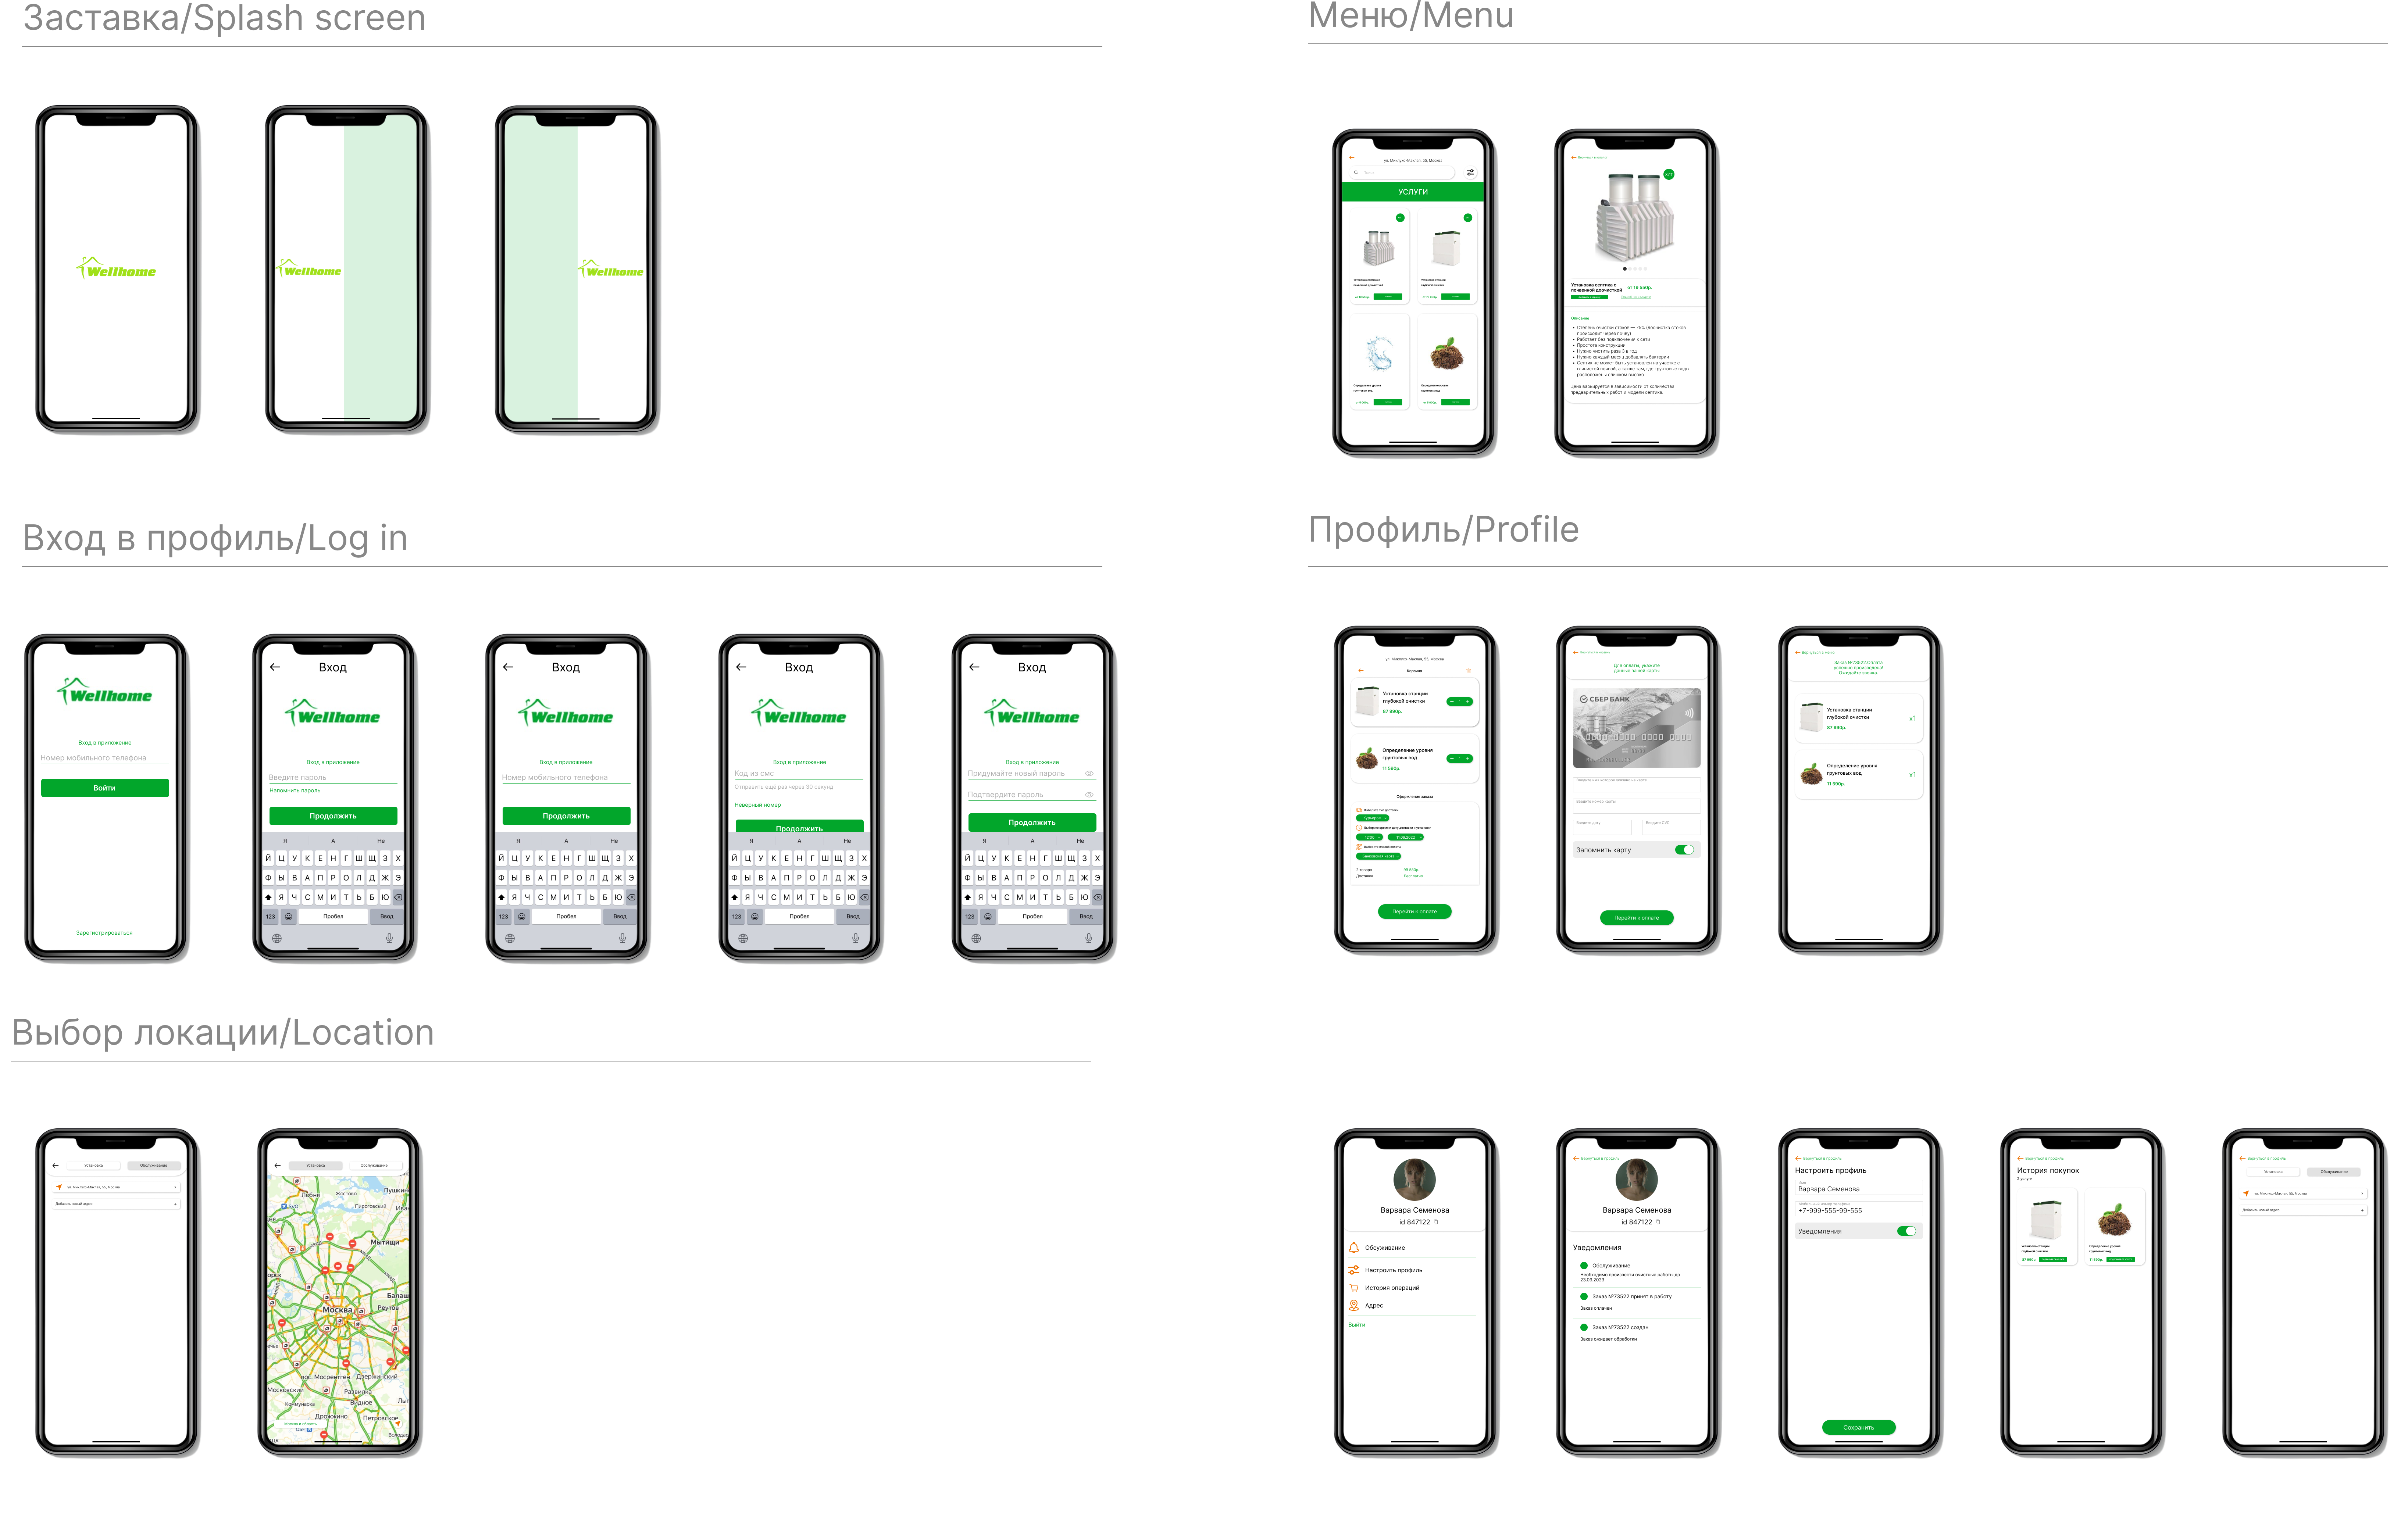
\includegraphics[width=\textwidth]{figma_all}
	\caption{Все экраны приложения}
	\label{figma_all}
\end{figure}

\subsection{Реализация пользовательского интерфейса}

\subsubsection{Средства разработки}

В основе всего приложения заложен архитектурный паттерн, применяемый при создании мобильных приложений, MVP --- Model View Presenter. По спроектированным макетам был разработан слой пользовательского интерфейса приложения, который и оказался реализацией слоя View.

В процессе создания приложения использовалась среда разработки XCode\cite{xcode}, предоставляющая весь необходимый функционал для написания кода на языке программирования Swift, реализации паттерна MVP, а самое главное --- открывающая возможность тестировать и запускать код на симуляторе мобильного устройства. 

Среда разработки и симулятор показаны на рисунке \ref{xcode}.

\begin{figure}[H]
	\centering
	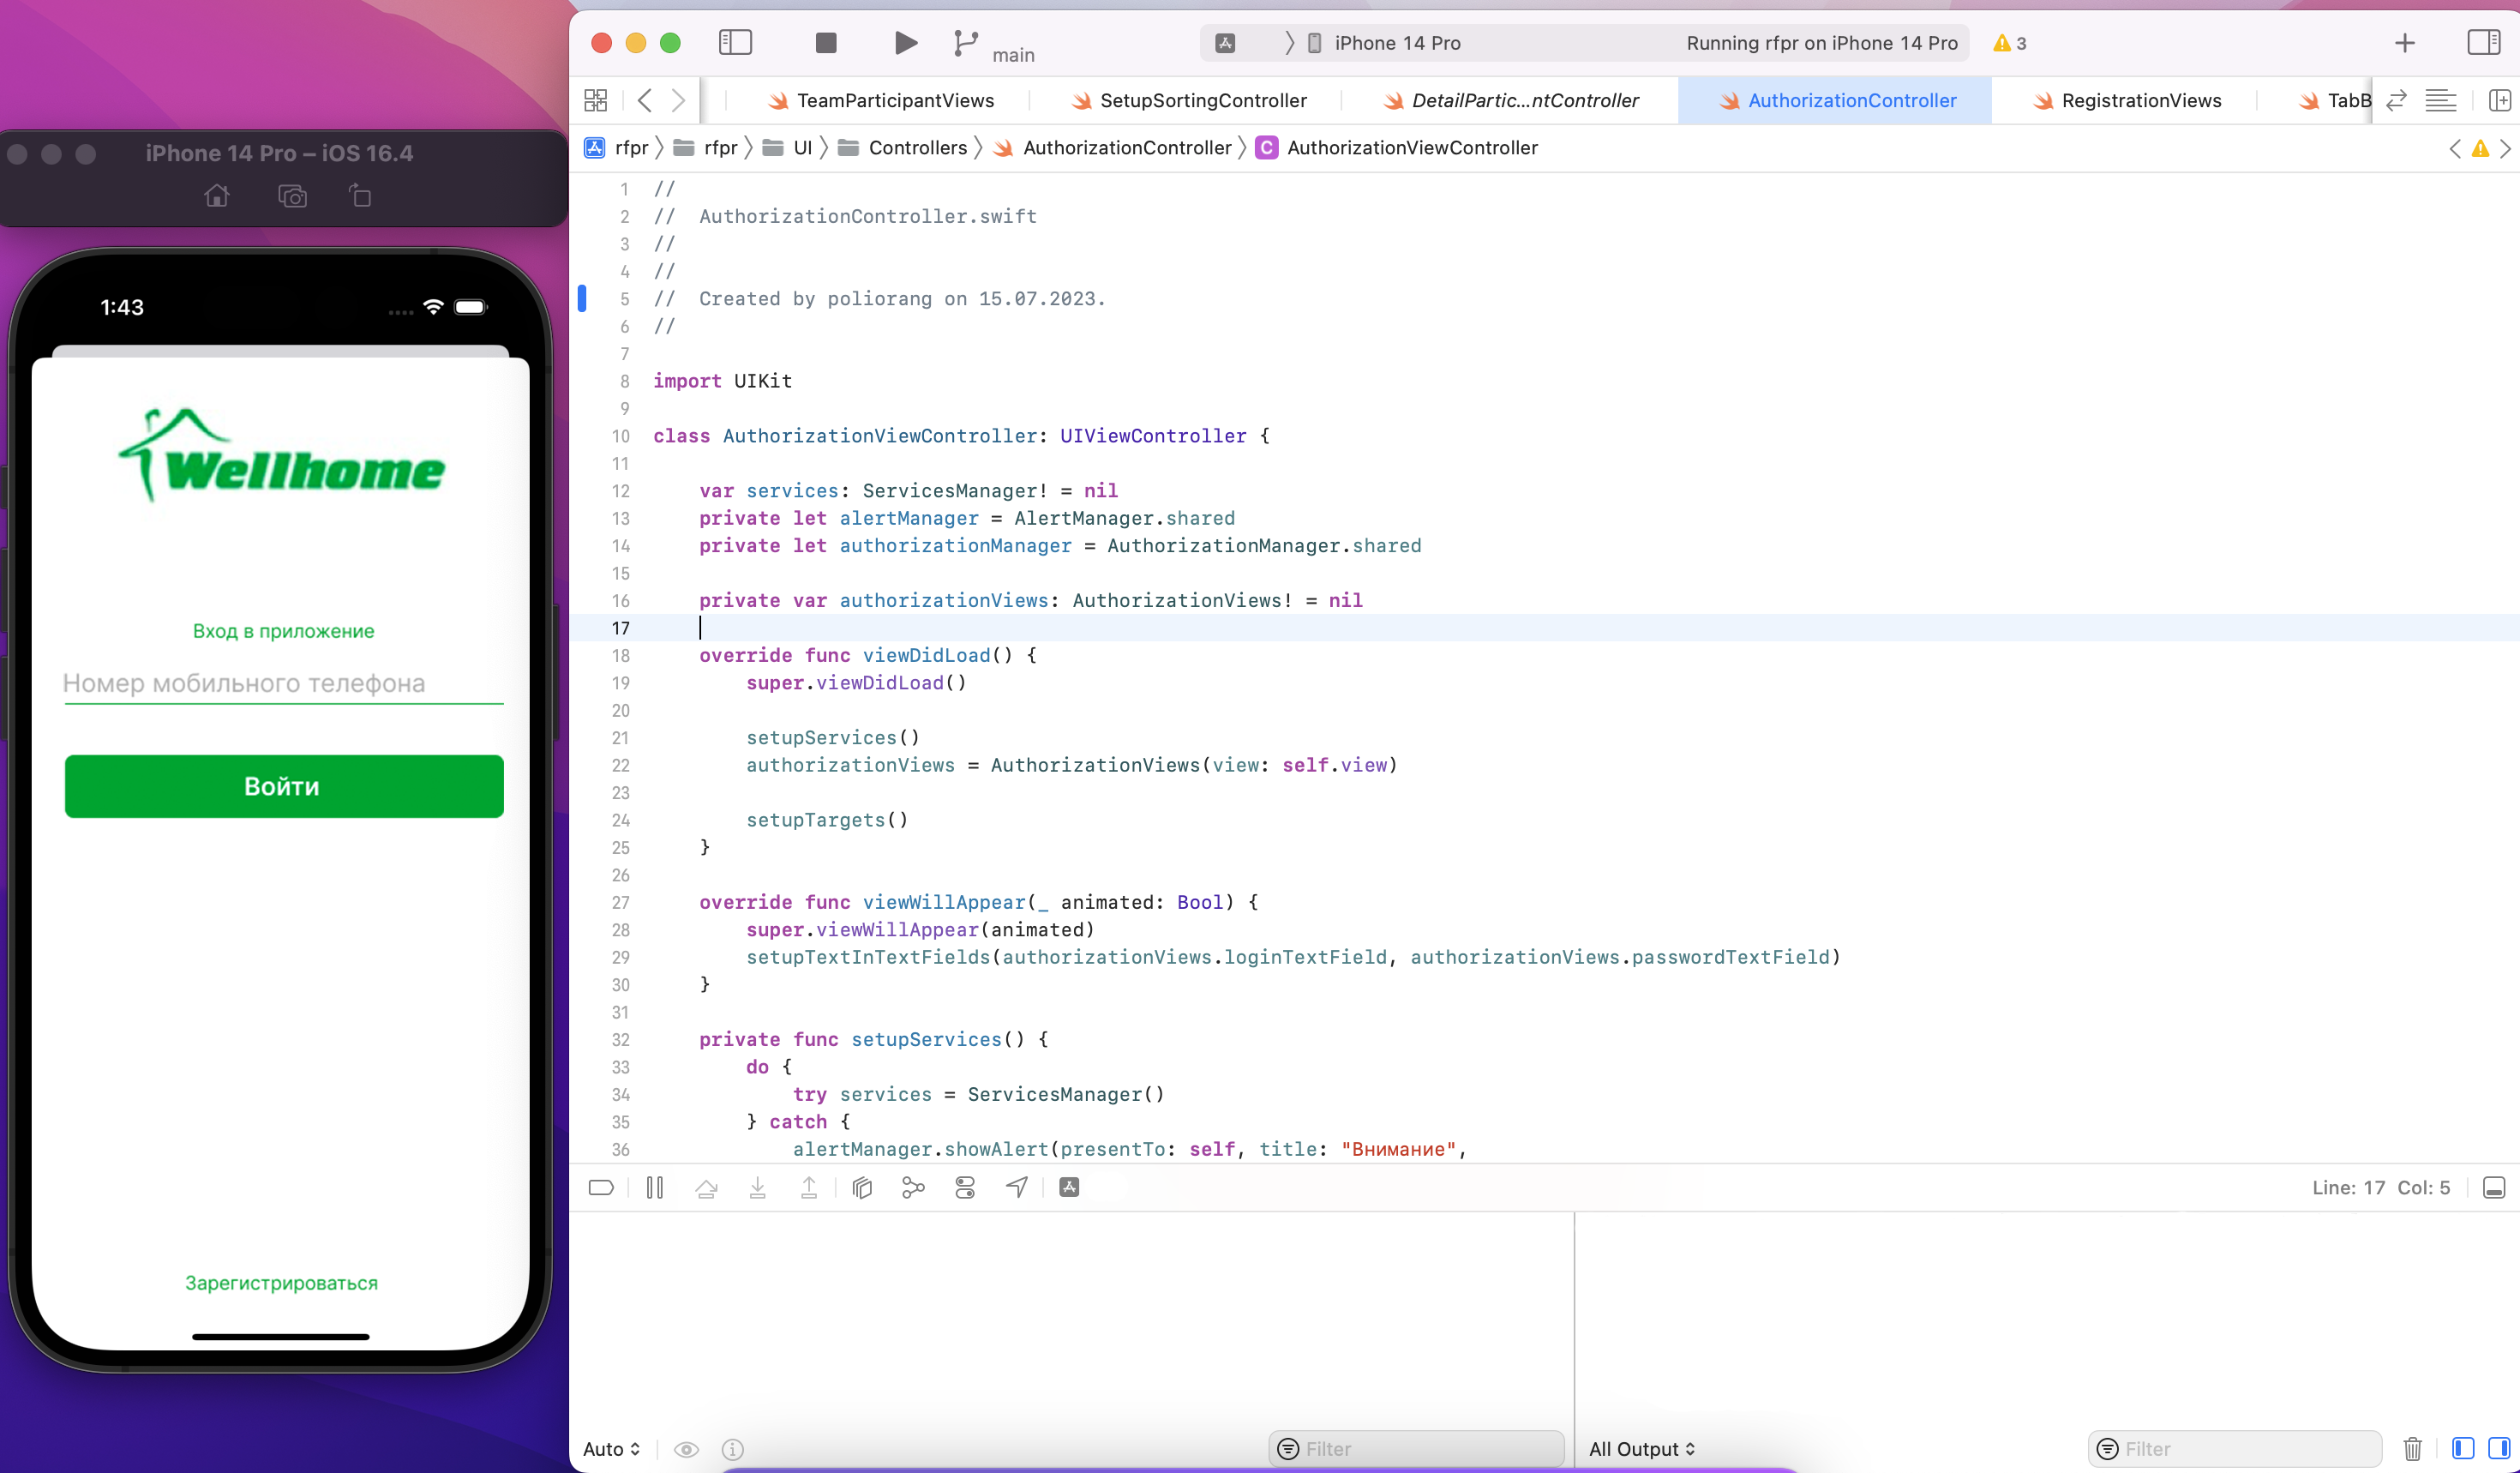
\includegraphics[width=\textwidth]{xcode}
	\caption{Среда разработки и симулятор }
	\label{xcode}
\end{figure}

\subsubsection{Разлизация}

Реализация начального экрана приложения показана на рисунке \ref{start_screen}.

\begin{figure}[H]
	\centering
	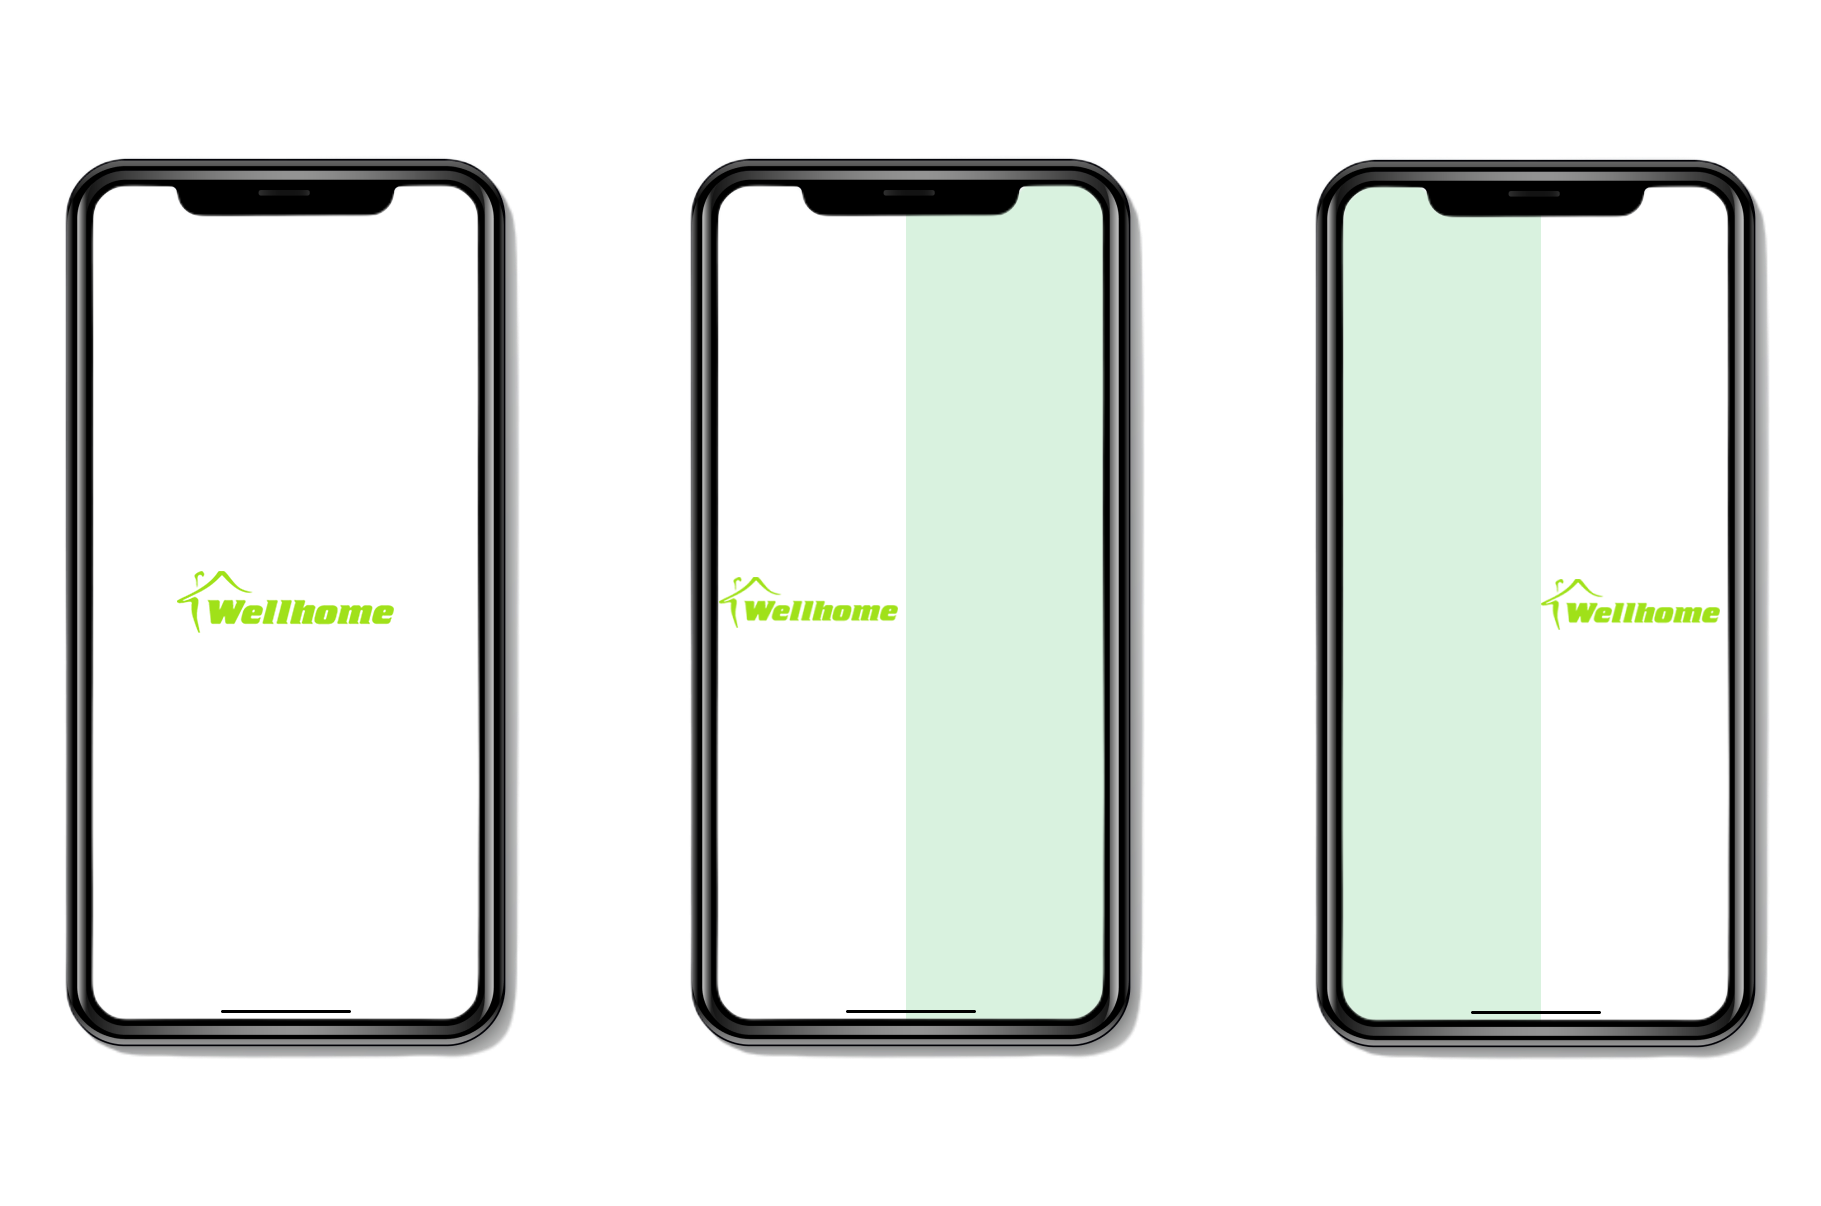
\includegraphics[width=\textwidth]{start_screen}
	\caption{Начальный экран приложения}
	\label{start_screen}
\end{figure}

Реализация экрана авторизации показана на рисунке \ref{login}.

\begin{figure}[H]
	\centering
	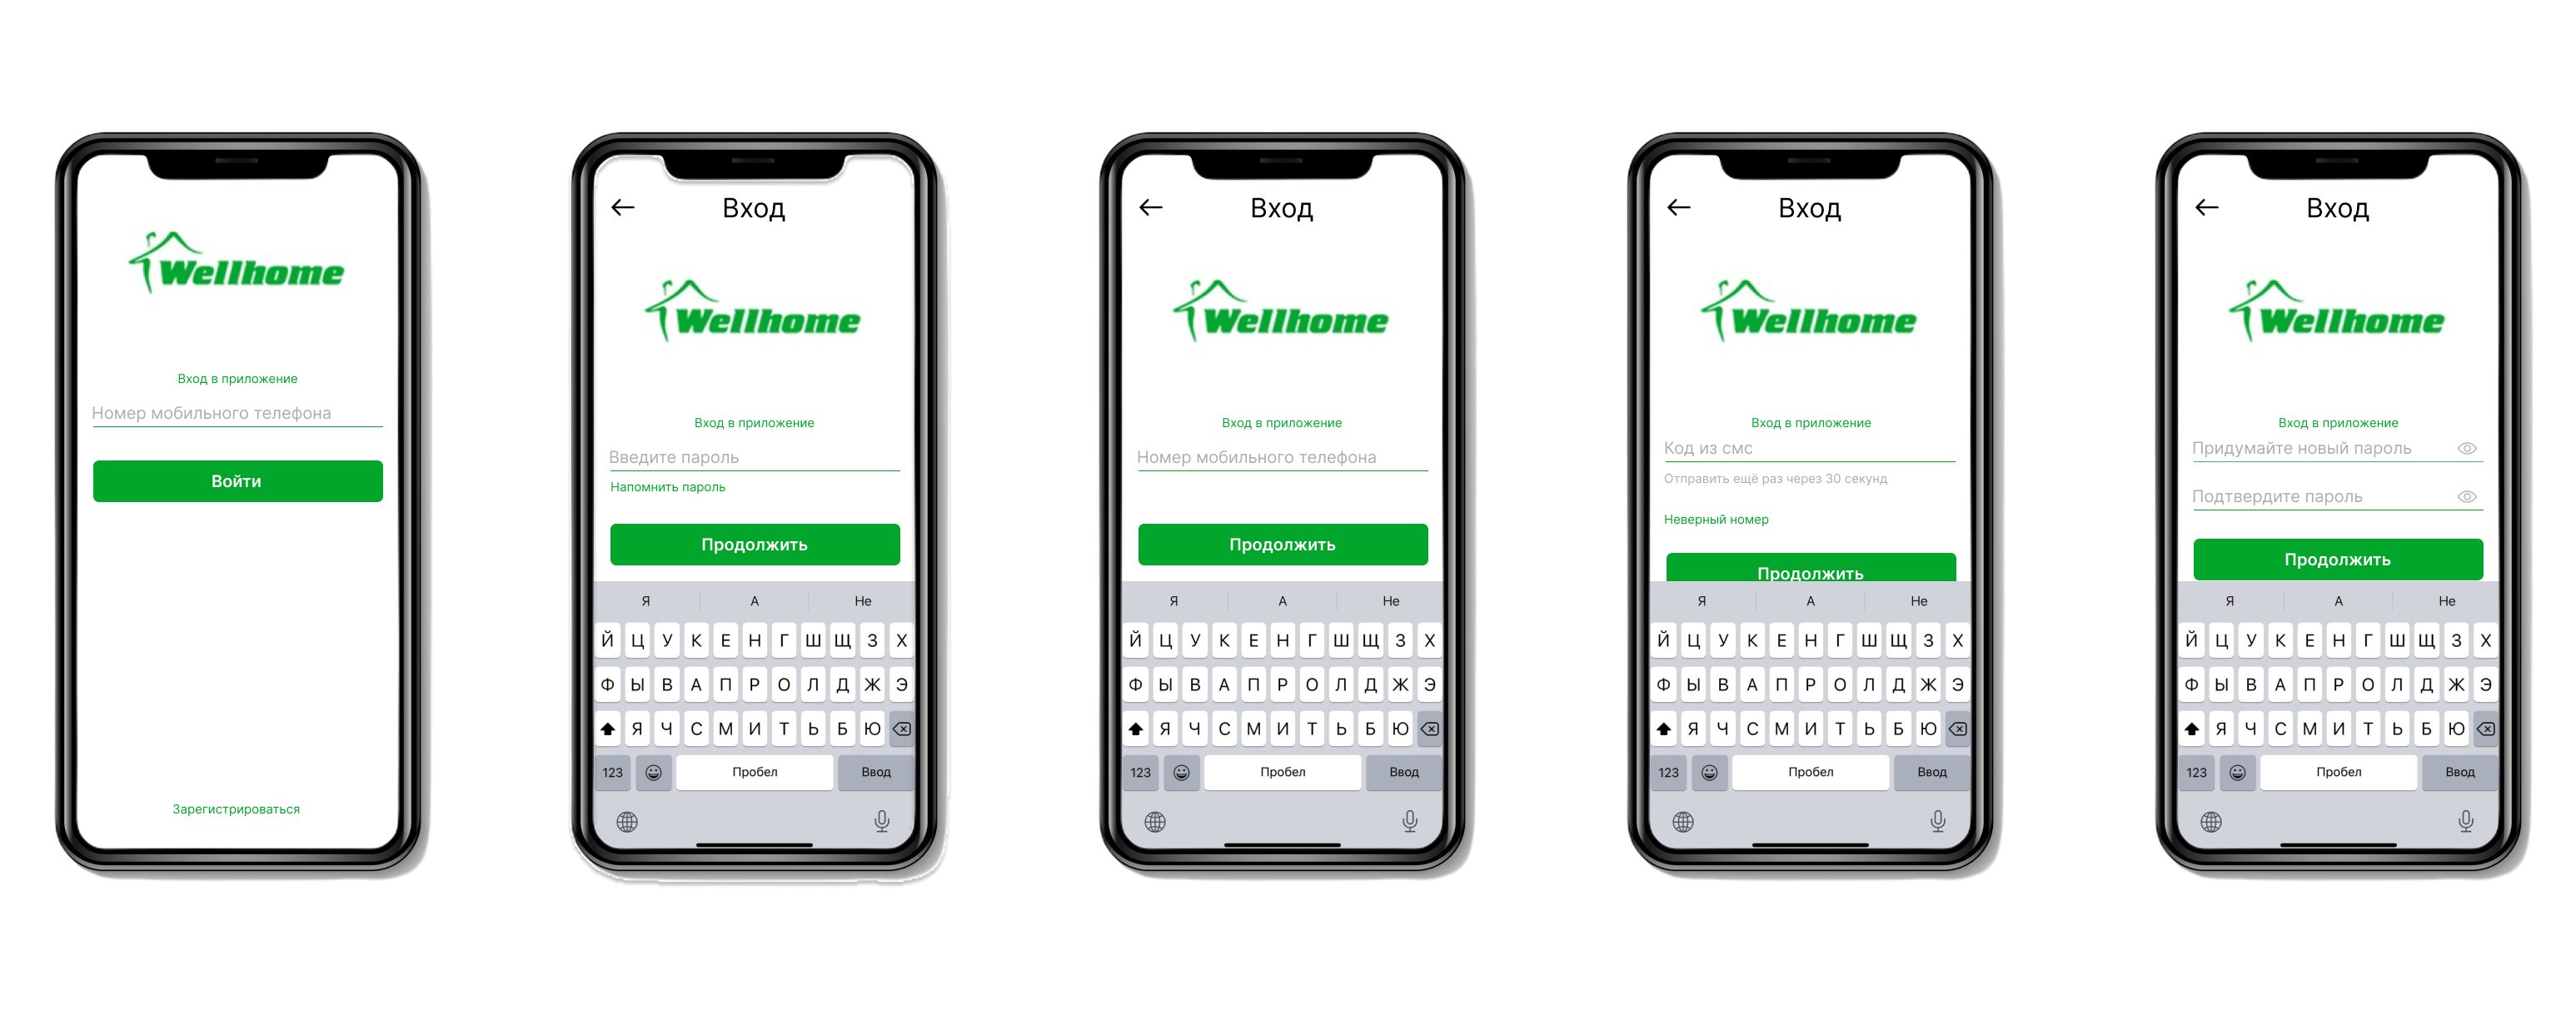
\includegraphics[width=\textwidth]{login}
	\caption{Экран авторизации}
	\label{login}
\end{figure}

Реализация экрана выбора локации показана на рисунке \ref{location}.

\begin{figure}[H]
	\centering
	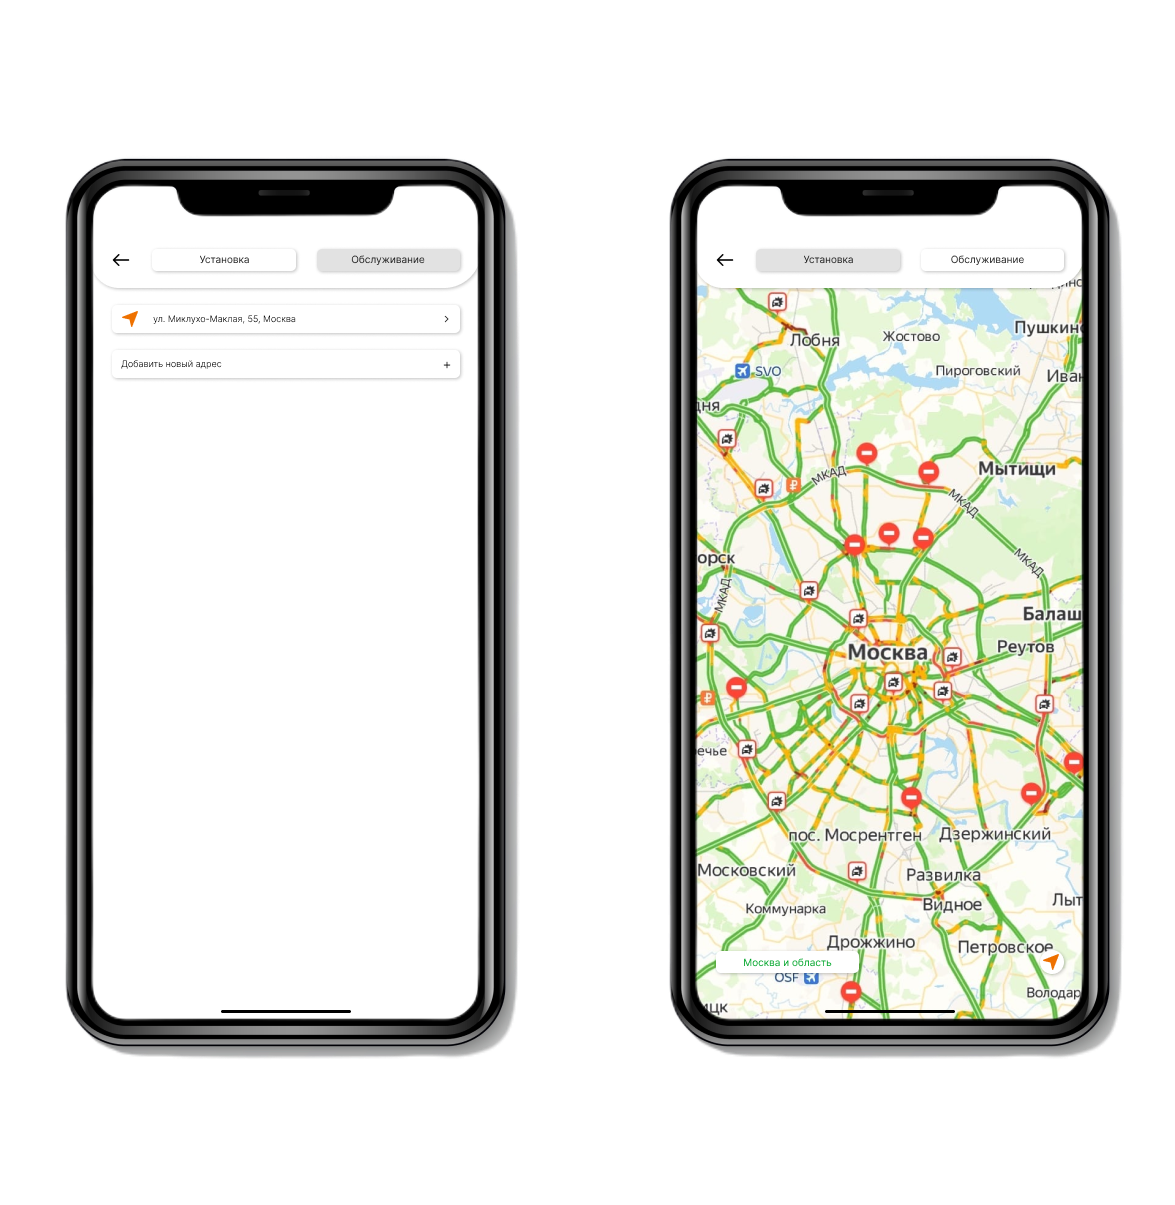
\includegraphics[height=300]{location}
	\caption{Экран выбора локации}
	\label{location}
\end{figure}

Реализация экрана поиска необходимой услуги и информации о ней показана на рисунке \ref{menu}.

\begin{figure}[H]
	\centering
	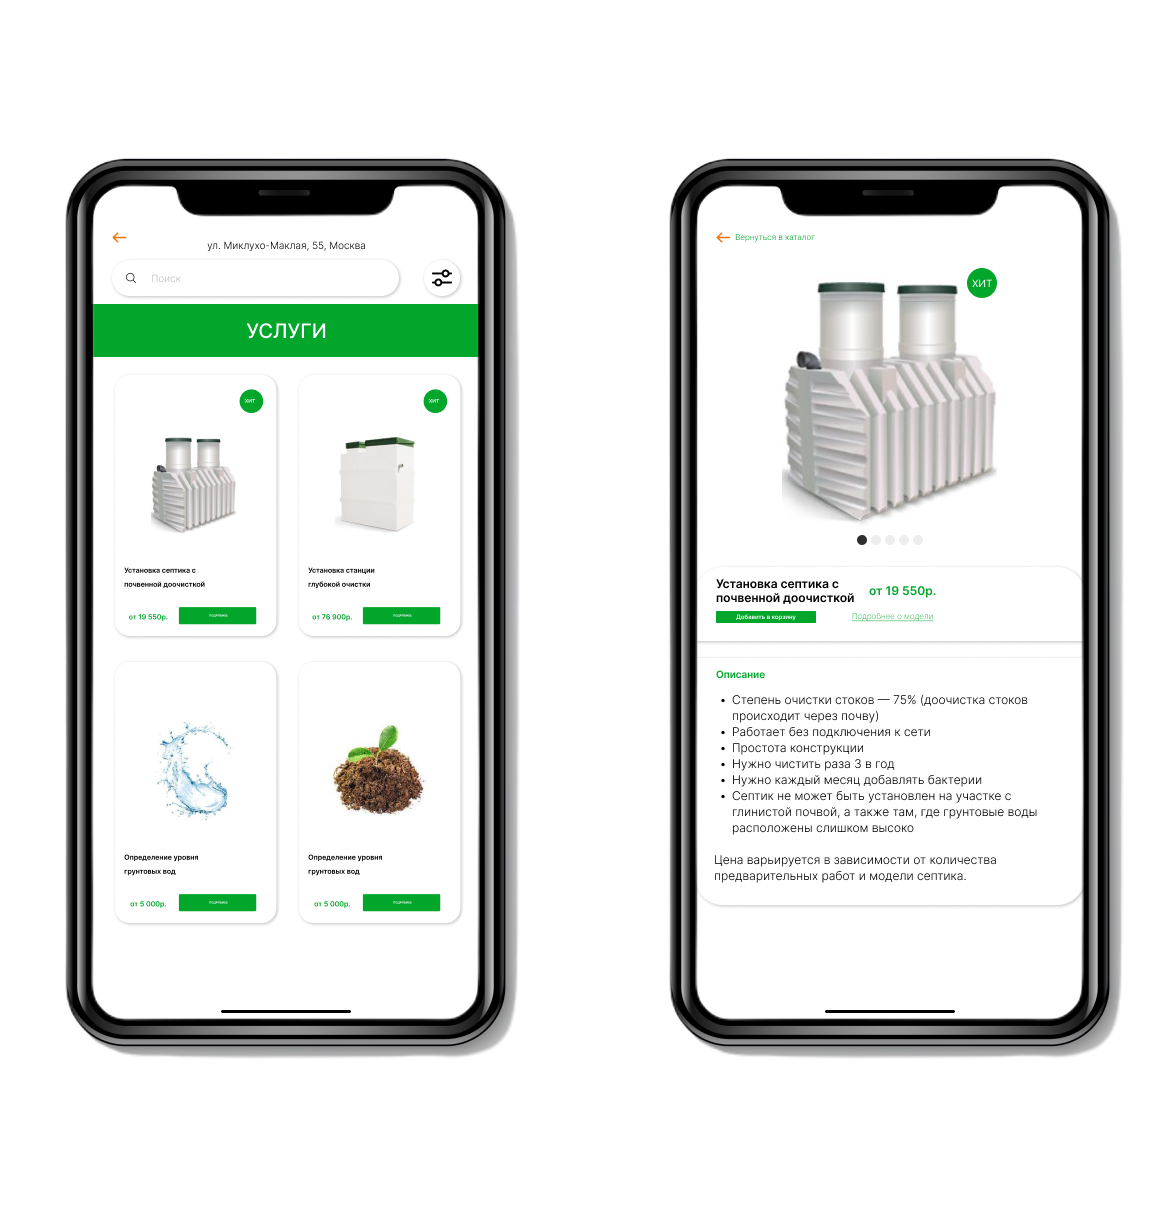
\includegraphics[height=300]{menu}
	\caption{Экран поиска услуги}
	\label{menu}
\end{figure}

Реализация экрана корзины клиента показана на рисунке \ref{basket}.

\begin{figure}[H]
	\centering
	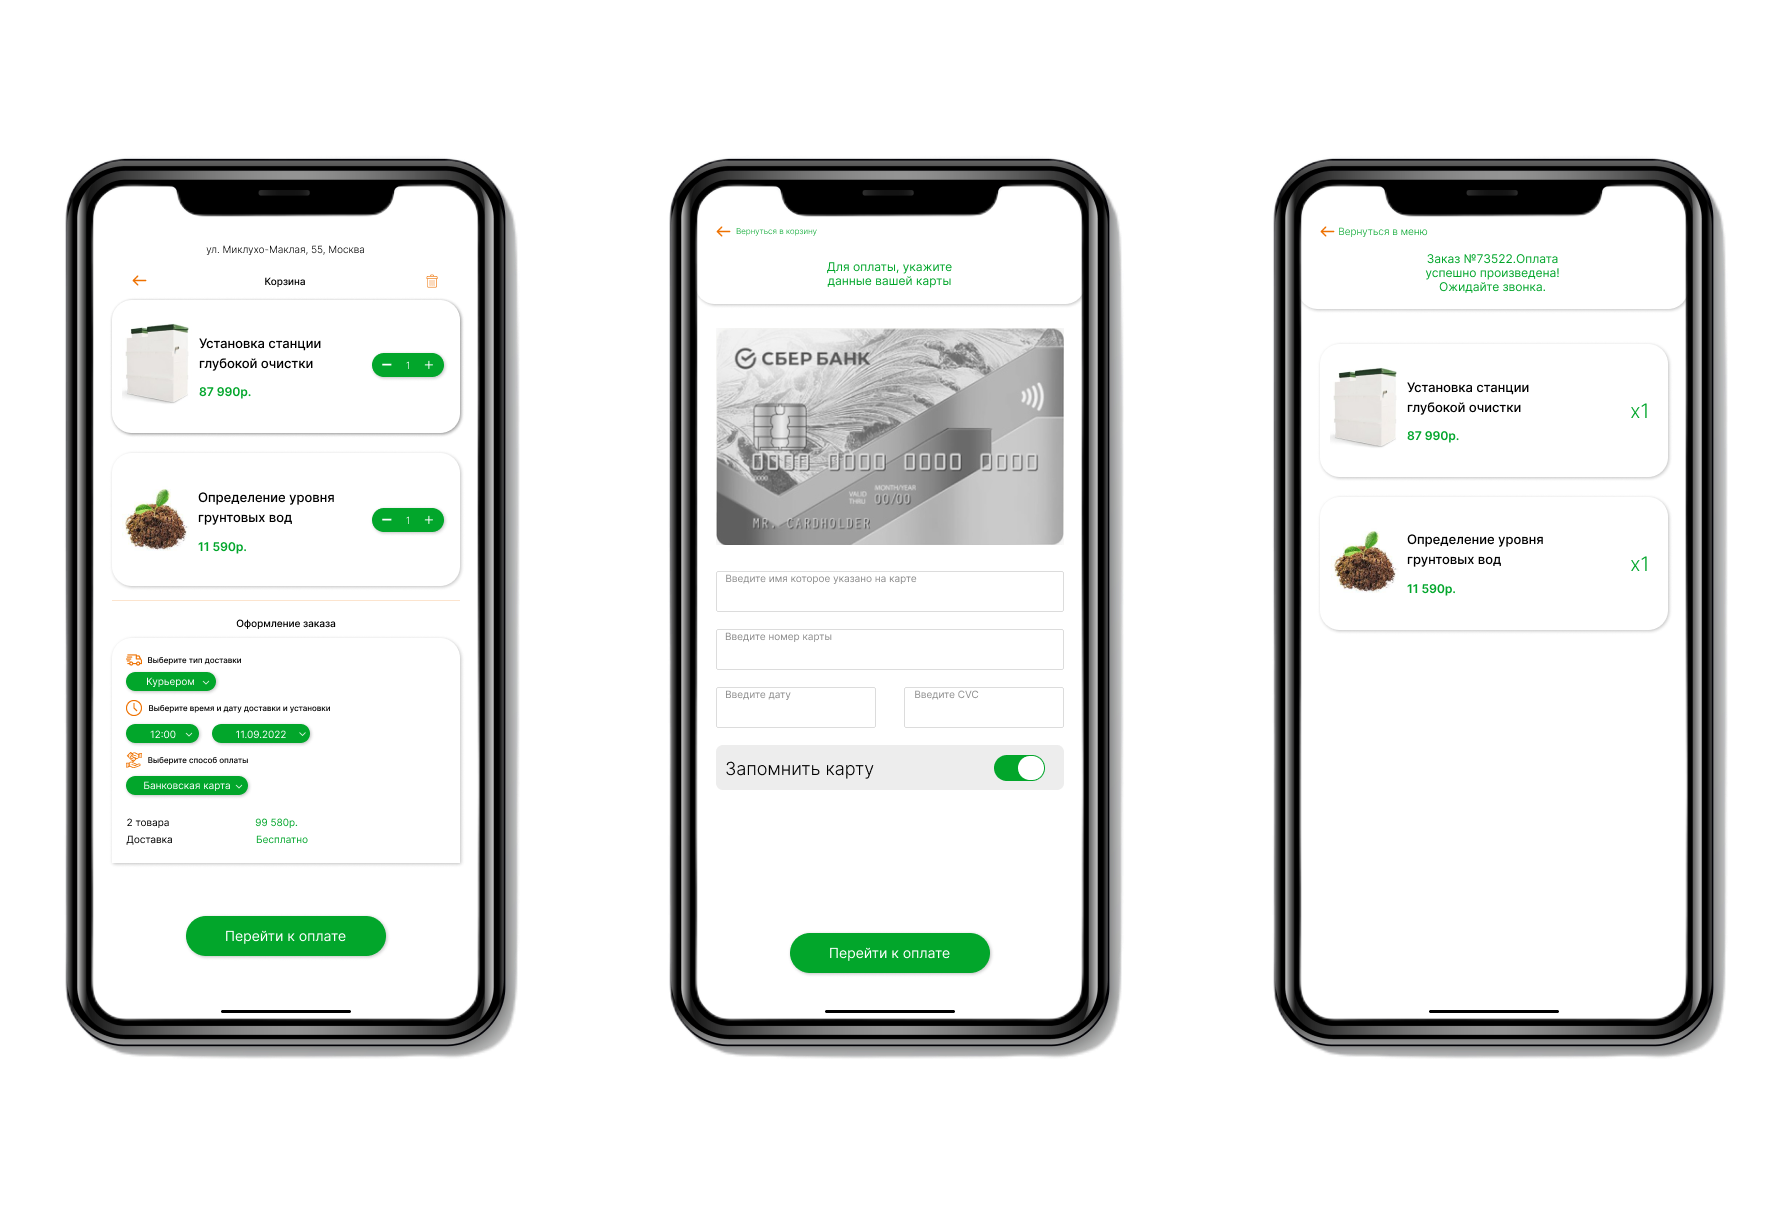
\includegraphics[width=\textwidth]{basket}
	\caption{Экран корзины клиента}
	\label{basket}
\end{figure}

Реализация экрана профиля показана на рисунке \ref{profile}.

\begin{figure}[H]
	\centering
	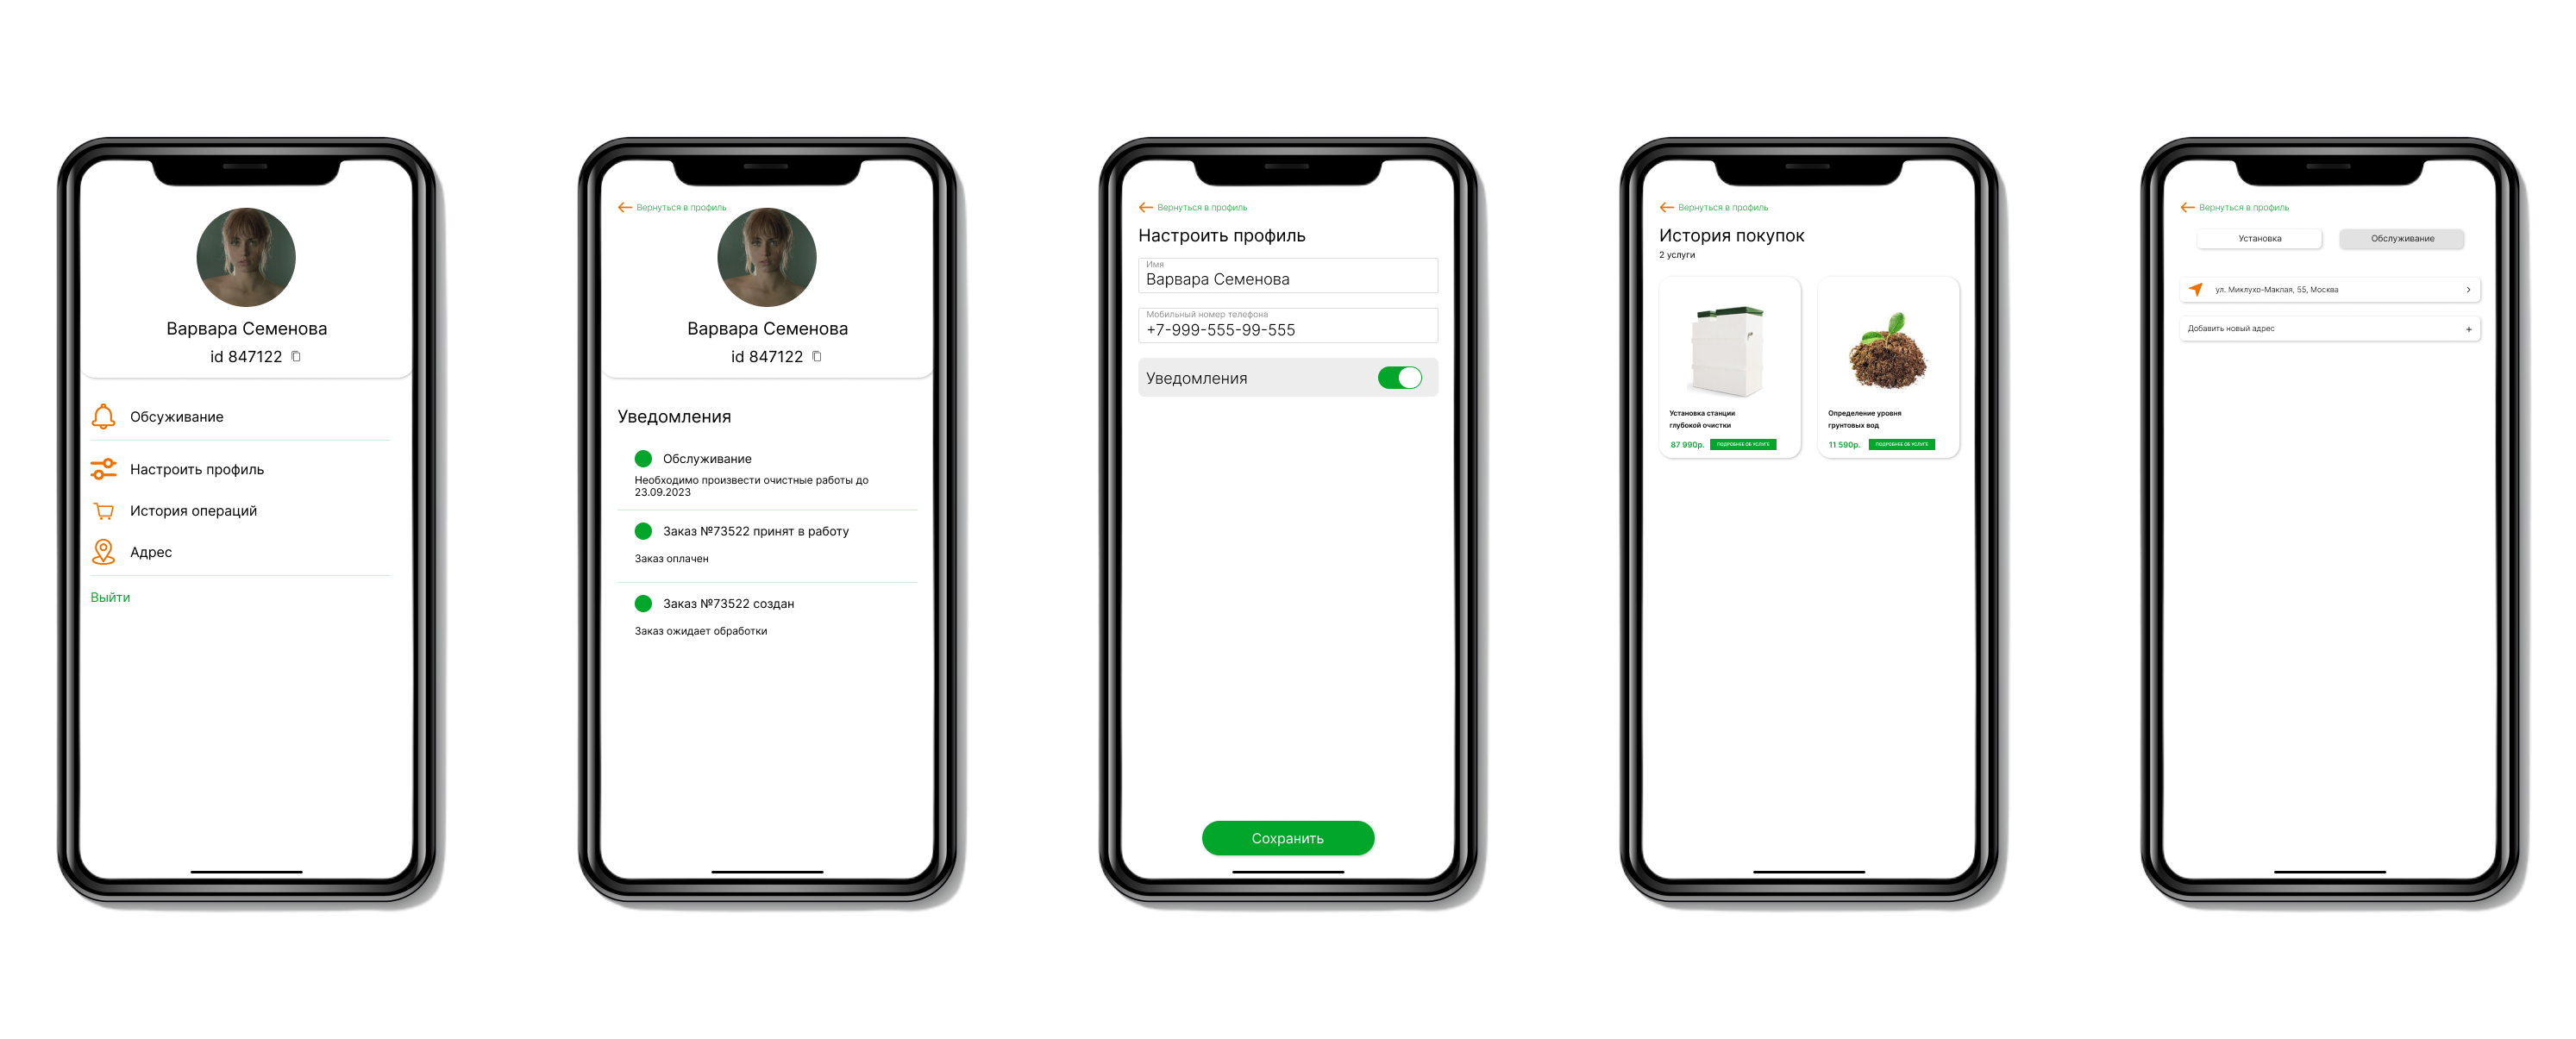
\includegraphics[width=\textwidth]{profile}
	\caption{Экран профиля}
	\label{profile}
\end{figure}

Поскольку при создании интерфейса приложения использовался метод AutoLayout фреймворка UIKit, слой UI масштабируем. Новые сотрудники в команде iOS--разработки смогут быстрее разобраться с уже имеющимся и кодом, чем, например, если бы проект был реализован при помощи InterfaceBuilder. В силу этого и добавление нового функционала будет происходить быстрее. 

\clearpage
